\section{Návrh metódy}
Navrhovaná metóda zohľadnuje vlastnosti, ktoré nie je možné získať iba zo statického obrazu, budeme ich nazývať dynamické príznaky videa.
Avšak metóda stále zohľadňuje v pozorovanom videu aj aspekty statického obrazu, tieto budeme nazývať statické príznaky videa.
Tieto príznaky sú vypočítavané separátne a nakoniec ich metóda spája do jednej výslednej mapy pozornosti. Výsledkom je postupnosť máp pozornosti pre každý frame videa (podľa vstupnej konfigurácie), ktorý možno spojiť do videa pozornosti pre ľubovolné vstupné video.

\subsection{Dynamické príznaky videa}
Dynamické príznaky metóda najprv extrahuje pomocou metódy Horn-Schunck\cite{horn-struct2}, ktorá vypočíta optický tok na každých 2 rozdielnych framoch videa, čím vzniká sémantický príznak pohybu rôznych objektov po scéne spolu s smerovými vektormi pohybu daných vektorov.
Získané smerové vektory okamžite spočítavame, aby sme získali celkový obraz optického toku pre danú dvojicu obrazov.
Obraz sa následne prahuje statickou konštantou kvôly ostráneniu šumu.
Prahovanie prebieha dynamicky vzľadom na počet nájdených 8-spojitých regiónov tj. výstup optikého toku. V našej implementácií je obmedzený počet regiónov na maximálnu hodnotu 200 regiónov.
Prahovanie začne s konštantou, ktorú určí pomocou algoritmu Otsu\cite{otsu}, následne určí počet 8-spojitých regiónov. Ak je počet väčší ako maximálna hodnota, zvýši konštantu o 10\% z pôvodnej hodnoty.
Tento proces sa opakuje pokial sa v obraze vyskytuje viac ako maximálny počet regiónov.
Takéto prahovanie je nutné pre optimalizáciu výkonu algoritmu, pretože v prípadoch keď obraz obsahuje veľké množtvo regiónov, výpočtová rýchlosť algoritmu je maximálne neúčinná.
Pixely s valídnou honotou sa rozdelia na regióny podľa spojitosti a podobnosti štandardným spôsobom.
Pripomenme, že v tomto obraze sa spočítali hodnoty posunu v oboch smeroch aritmeticky do jednej hodnotiacej konštanty (pre každý pixel obrazu), ktorá už nereprezentuje smer posunu daného obrazového pixelu, ale iba hodnotí celkový posun pixelu.
Takto získané regóny budeme vyhodnocovať a spájať podľa pôvodných výsledkov metódy Horn-Schunck.
Vďaka využitiu pôvodných vektorov z výsledku metódy Horn-Schunck, vieme rozlíšiť pohyb horizontálny aj vertikálny separátne.
Pre všetky dvojice regiónov v obraze zisťujeme nasledovné charakteristiky:
\begin{enumerate}
  \item\textbf{Rozdiel smerových vektorov v horizontálnom smere}
  \item\textbf{Rozdiel smerových vektorov v vertikálnom smere}
  \item\textbf{Rozdiel vo vzdialenosti}
\end{enumerate}
\subsubsection{Rozdiel smerových vektorov v horizontálnom smere}
Charakteristika sa vypočítava zo smerových horizontálnych vektorov metódy Horn-Schunck.
Pre každý región sa vypočíta maximálna hodnota z indexov daného regiónu.
Následne sa za hodnotu chrakteristiky sa považuje absolútna hodnota rozdielu týchto hodnôt pre každý región.
\begin{equation}
  H_A = max(HS(i_A))
\end{equation}
\begin{equation}
  H_B = max(HS(i_B))
\end{equation}
\begin{equation}
  R_{H} = abs(H_A-H_B)
\end{equation}
Kde A, B reprezentujú všetky dvojice regiónov, ktoré sa nachádzajú v obraze.
\begin{math}V_a, V_b\end{math} je maximálna hodnota horizontálnych smerových vektorov z výsledku Horn-Schunck algoritmu pre všetky oblasti patriace danému regiónu.
\begin{math}R_{H}\end{math} je výsledná hodnota charakteristiky.

\subsubsection{Rozdiel smerových vektorov v vertikálnom smere}
Charakteristika sa vypočítava zo smerových vertikálnych vektorov metódy Horn-Schunck.
Pre každý región sa vypočíta maximálna hodnota z indexov daného regiónu.
Následne sa za hodnotu chrakteristiky považuje absolútna hodnota rozdielu týchto hodnôt.

\begin{equation}
  H_A = max(HS(i_A))
\end{equation}
\begin{equation}
  H_B = max(HS(i_B))
\end{equation}
\begin{equation}
  R_{V} = abs(H_A-H_B)
\end{equation}
Kde A, B reprezentujú všetky dvojice regiónov ktoré sa nachádzajú v obraze.
\begin{math}V_a, V_b\end{math} je maximálna hodnota vertikálnych smerových vektorov z výsledku Horn-Schunck algoritmu pre všetky oblasti patriace danému regiónu.
\begin{math}R_{V}\end{math} je výsledná hodnota charakteristiky.

\subsubsection{Rozdiel vo vzdialenosti}
Chrakteristika sa vypočítava ako minimálna hodnota vzdialenosti medzi dvojicou regiónov.
Hodnota je počítaná euklidovskou metódou.

\begin{figure}[H]
  \begin{algorithm}[H]
   \ForAll{rohA ako každý extrém regiónu A}{
     \ForAll{rohB ako každý extrém regiónu b}{
      vzdialenosť = sqrt( (corner2(1,1)-rohB(1,1))^2 + (rohB(1,2)-rohA(1,2))^2 ) \\
     }
   }
   \caption{Výpočet minimálnej vzdialenosti euklidovskou metódou}
  \end{algorithm}
  \vspace{10mm}
\end{figure}

\subsubsection{Spájanie regiónov}
Po výpočte všetkých 3 charakteristík spojíme všetky dvojice regiónov, pre ktoré sú všetky chrakteristiky nižšie ako zadefinovaná konštanta.
Regióny spájame pomocou konvexného obalu zjednotenia bodov ležiacich v oboch regiónoch.
\begin{figure}[H]
  \centering
  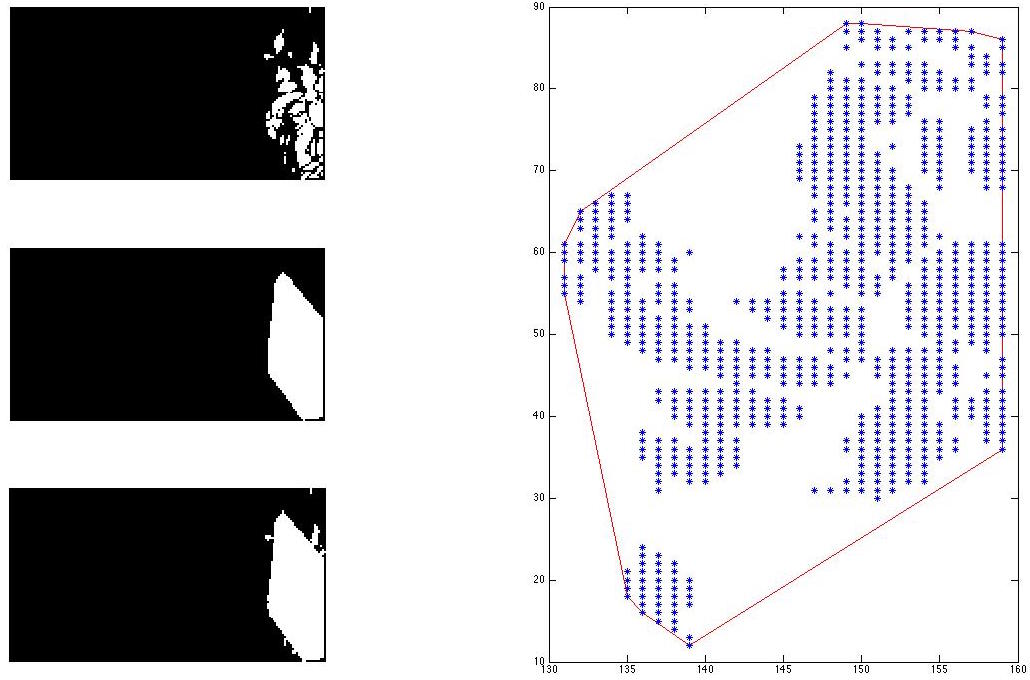
\includegraphics[width=15cm]{pics/spojenie-regionov.jpg}
  \caption{Vizualizácia spojenia regiónov pomocou konvexného obalu}
  \vspace{10mm}
\end{figure}

\subsubsection{Starnutie objektov na scéne}
Do vypočitavania dynamických príznakov započítavame predpoklad, že aj pohybujúce sa objekty postupne strácajú pozornosť používateľov.
A to v prípade kedy sa síce daný objekt na scéne pohybuje, ale na identickom mieste.
Do metóty zabudujeme mechanizmus, kde pixelom s dlhodobo vysokým hodnotením pozornosti, zmenšíme toto hodnotenie pomocou  vynásobenia koeficientom hodnoty \numrange{0}{1}.

\subsection{Statické príznaky videa}
Pri videách, kde sa pohybuje celá scéna (kamera je v pohybe) nedávajú dynamické príznaky dobré výsledky keďže logicky označia celú scénu alebo väčšinovú časť scény za výrazne salientnú.
Preto je vhodné dynamické príznaky vhodne kombinovať s klasickými modelmi pozornosti, ktoré síce zanedbajú postupnosť obrazov, ale nezlyhajú ako dynamické príznaky.
Pre extrakciu statických obrázkov sme zvolili metódu založnú na spektralnych reziduach\cite{spectral-rezidual}.
Vďaka svojmu príncípu potlačovania štatisticky opakujúcich sa predmetov na scéne, sa dá predpokladaď vhodné doplnenie statických objektov, ktoré môžu zaujať pozornosť na videu ak zlyhávajú dynamické príznaky.

\subsection{Výsledné spojenie príznakov}
Spájanie dynamických a statických príznakov bude prebiehat pomocou sčítania oboch máp, pričom vždy sa použijú v určitom pomere.
Výpočet pomeru bude určovať pomer výskytu salientných pixelov v mape dynamických príznakov.

\begin{equation}
pomer = \sum_{n=0}^{Pix_{count}} P_D(n) > 0 / Pix_{count}
\end{equation}
\\
Kde \begin{math}P_D\end{math} reprezentuje mapu dynamických príznakov a \begin{math}Pix_{count}\end{math} je počet všetkých pixelov, ktoré obraz obsahuje.

Ak je vysoký výskyt salientých pixelov, potrebujeme utlmiť zobrazovanie tejto časti príznakov a prioritizovať zobrazovanie statických priznakov, preto zmiešavacia funkcia vyzerá nasledovne:

\begin{equation}
  Výsledok = (P_D * (1-pomer)) + (P_S * pomer)
\end{equation}
Kde \begin{math}P_D\end{math} reprezentuje mapu dynamických príznakov a \begin{math}P_S\end{math} mapu statických príznakov.

V prípade, že algoritmus nedokáže detekovať žiadny pohyb na scéne, bol by model pozornosti prázdny.
Preto v prípade, keď je vyššie spomýnaný pomer dynamických pixelov extrémne nízky použijeme ako výstup algoritmu iba statické príznaky.
Naopak v prípade, že kamera je v pohybe Horn-Schunck algoritmus označí ako pohybujúci sa väčšinovú oblasť obrazu a v tom prípade je potrebné utlmiť dynamické príznaky obrazu a do popredia vystupujú statické.

\subsection{Zdrojové kodý modelu}
Zdrojový kód obsahuje jednu metódu, ktorá príjima na vstupe vždy 2 parametre.
Prvý parameter je aktuálny frame videa a druhý parameter je frame videa určený na extrakciu dynamických príznakov videa pomocou differencie vzľadom na prvý obrazový frame.
Tieto 2 obrazové vstupy nemusia byť nutne po sebe idúce, je na používateľovi či použije model serializovane na každý frame videa, alebo zvolí vlastnú implementáciu keyframingu (napríklad kvôly časovej náročnosti algoritmu).
Algoritmus je schopný processovať farebné aj čiernobiele obrazové vstupy.
V prílohe je možné nájsť 2 implementácie a to implementáciu modelu pre applikáciu na porovnávanie modelov načítavajúca kažké 2 posebeidúce obrazové framy.
Druhá implementácia načítava na vstupe priamo video a na výstup dá video s korešpondujúcim videom význačných oblastí, tátoimplementácia je určená na použitie mimo aplikácie na testovanie.
Obe implementácie sú dostupné v prílohe na CD alebo voľne dostupné na internete.

\subsection{Ukážky výsledkov}
V tejto sekcií budem prezentovať výsledky konkrétne prípady videí (framy) zachytené počas testovania a validácie.
Uvediem po sebe nasledujúce originálne framy videa a vizualizáciu fixácií. Ako príklad uvediem frame 53 z videa č. 23 z datasetu ASCMN\cite{accv}.
\begin{figure}[H]
  \centering
  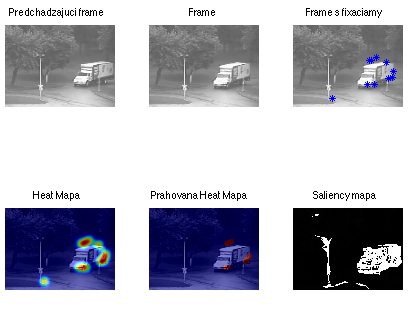
\includegraphics[width=10cm]{pics/ACCV-23-54-compare.png}
  \caption{Porovnanie výstupu mapy pozornosti a reálnych dát}
  \label{fig:ASCMN-53-23}
  \vspace{10mm}
\end{figure}
Grafy sú generované pomocou pozmeneného ukážkového scriptu distribuovaného spolu s datasetom ASCMN\cite{accv} a porovnávané s výsledkom navrhovaného modelu pomocou grafu \ref{fig:ASCMN-53-23}.
V prvom riadku vidíme ako prvý pôdovdný frame (n-1) nasledovaný testovaným framom a posledný obrázok zobrazuje fixácie.
V druhom riadku uvádzam postupne heatmapu pre daný frame, prahovanú heat mapu a ako poslednú výslednú saliency mapu.

\begin{figure}[H]
  \centering
  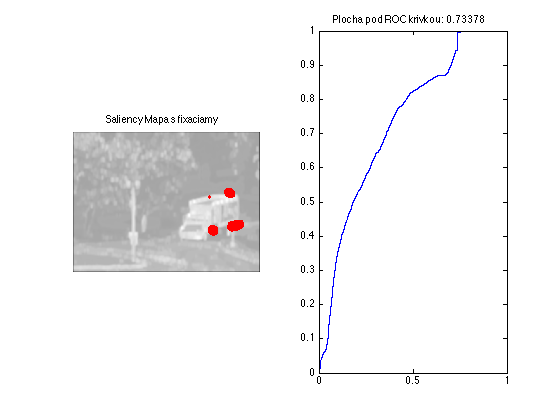
\includegraphics[width=10cm]{pics/ACCV-23-54-AUC_Judd.png}
  \caption{Vizualizácie metriky AUC-Judd pomocou kódu zverejneného v mit saliency benchmark\cite{mit-saliency-benchmark}}
  \label{fig:ASCMN-53-23-AUC}
  \vspace{10mm}
\end{figure}

Z grafov \ref{fig:ASCMN-53-23} vidno koreláciu dát, čo taktiež povrdzuje metrika vypočítaná na danom frame na grafe \ref{fig:ASCMN-53-23-AUC} reprezentujúca AUC-Judd\cite{auc-judd} krivku.

\subsubsection{Problémové typy videí}
V tejto sekcií uvediem typové video s rovnakou analýzov ako je uvedená vyššie, iba na typ videa bude nevhodný navhovaný model.
Typovo videá možno označit ako videá s fixovanou kamerou v pohybe.
Tj. kamera je fixovaná k sledovanému objektu na scéne, z čoho vyplýva, pozadie obrazu (okolie sledovaného objektu) je pre náš algoritmus v pohybe aj keď reálne sa hýbe kamera a preto je považované za významný objekt.
Zároveň sledovaný objekt (často aj objekt v pozornosti používateľov) sa vizuálne nepohybuje, z dôvodu, že jeho pohyb je kompenzovaný fixáciou kamery a preto ho navrhovaný algoritmus povazuje za vyzuálne nevýznamný.
Ako príklad uvediem frame č.80 z videa č. 10 z datasetu coutrot #1.

\begin{figure}[H]
  \centering
  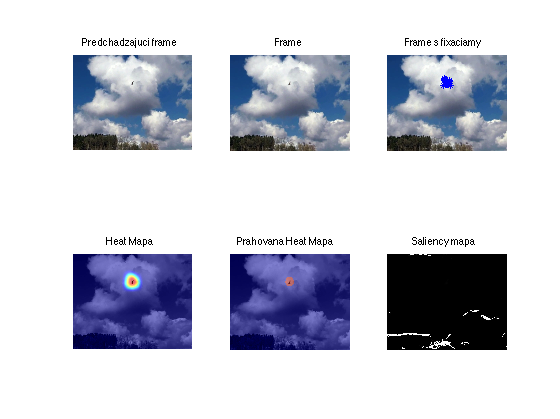
\includegraphics[width=10cm]{pics/bad-compare.png}
  \caption{Porovnanie výstupu mapy pozornosti a reálnych dát}}
  \label{fig:coutrot-bad}
  \vspace{10mm}
\end{figure}

Už podľa grafu \ref{fig:coutrot-bad} nemá výsledok navrhovaného modelu žiadnu koreláciu s reálnymy dátamy.
Preto nebudeme dalej uvádzať žiadnu metriku.
Návrh riešenia pre tieto prípady budú rozanalyzované v sekcií \ref{ssec:diskusia}.

\clearpage

\subsection{Pipeline metódy}
  Grafický popis metódy obsahujúci graf zostavenia mapy pozornosti.

  \begin{figure}[H]
    \centering
    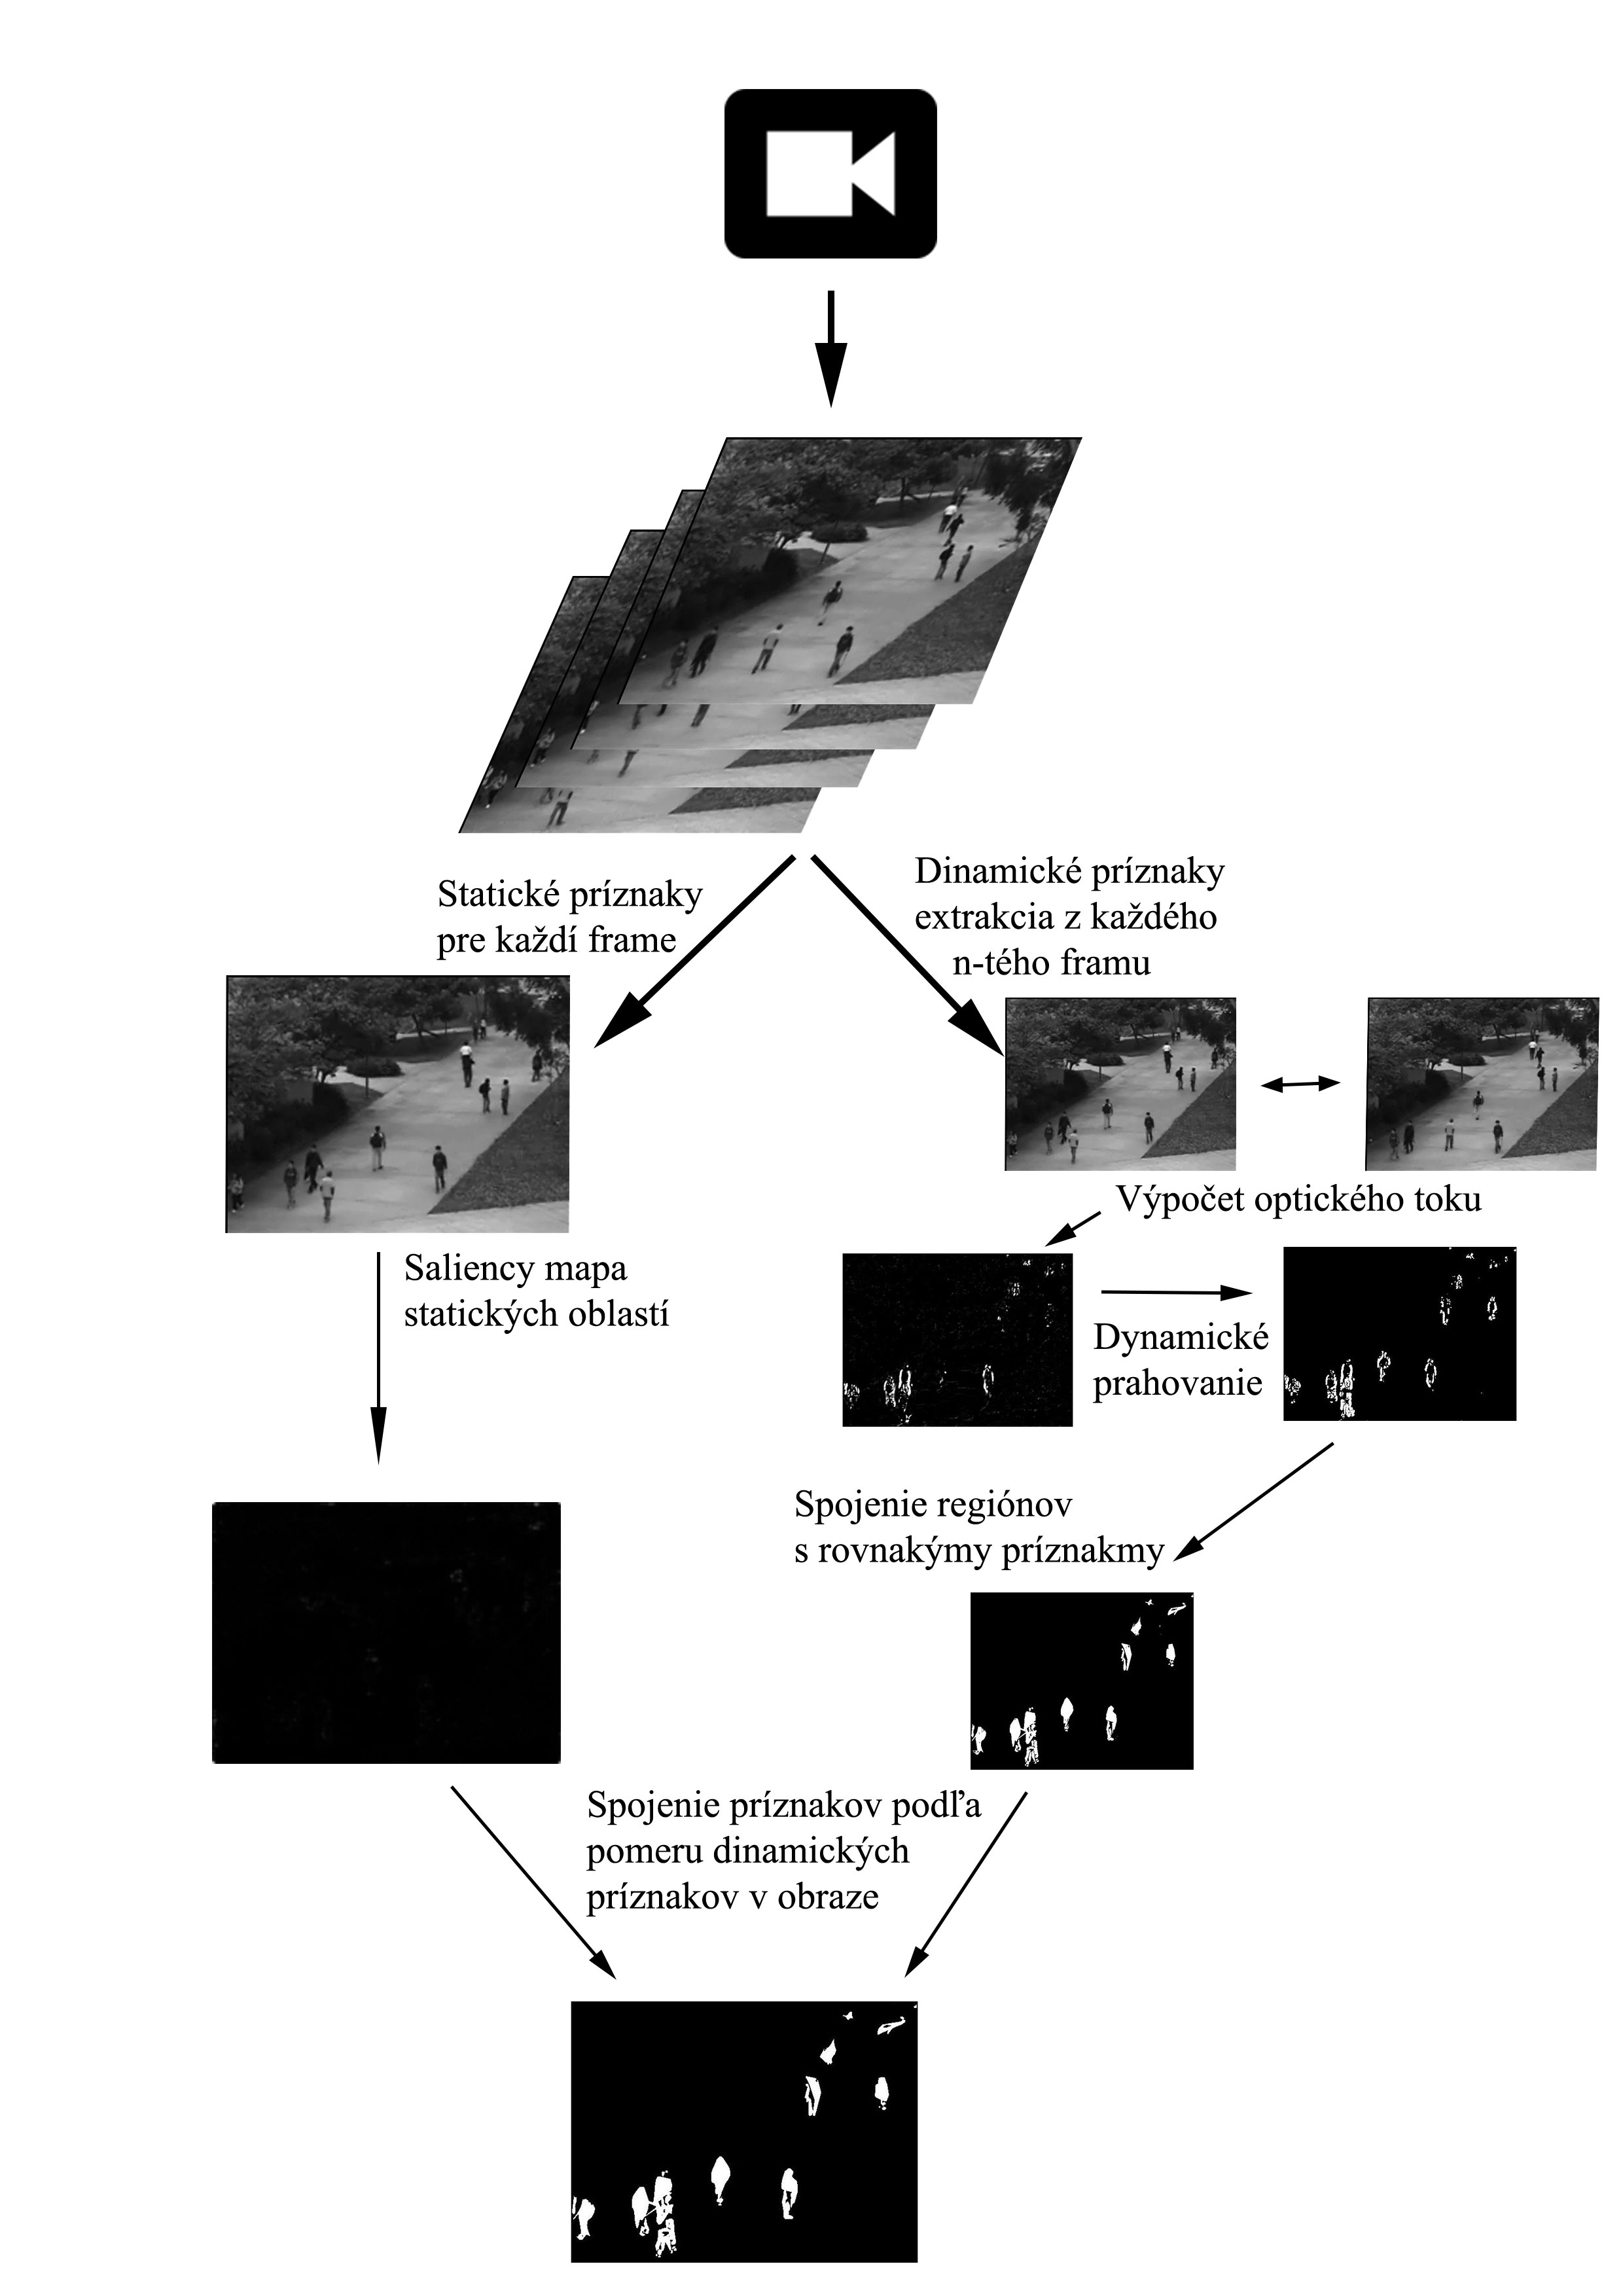
\includegraphics[width=15cm]{pics/workflow.jpg}
    \caption{Ucelená vizualizácia algoritmu}
    \vspace{10mm}
  \end{figure}

\section{Implementácia riešenia}
Implementácia vyššie uvedeného algoritmu je implementovaná ako modul pre aplikáciu na porovnávanie a  automatickú validáciu výsledkov.
Aplikácia na porovnávanie je takisto implementovaná v prostredí matlab.

\subsection{Aplikáciu na porovnávanie a automatickú validáciu}
Sekundárnym prínosom práce je vytvorenie aplikácie pre zjednodušenie budúcej práce pri prototypovaní nových modelov pozornosti.
A následné uľahčenie validačného procesu pre potencionálnych vývojárov.\\
Základná functionalita:
\begin{enumerate}
  \item\textbf{Oddelenie logiky testovania a logiky samotného modelu}
  \item\textbf{Simultálne sledovanie videa z viacerých modelov}
  \item\textbf{Automatická validácia modelu}
  \item\textbf{Vizualizácia výsledkov validácie}
\end{enumerate}

\subsubsection{Oddelenie logiky testovnia a logiky samotného modelu}
V aplikácií na testovanie je možné pridávať ľubovolné modely, pre ktoré je dostupná implmentácia v jazyku matlab.
Pre iné jazyky je potrebné doprogramovať wrapper, ktorý spustí daný jazyk a vypočíta mapu pozornosti.
Ukážkový wrapper je súčasťou aplikácie.
Pre pridanie nového modelu je potrebné pridať wrapper do zložky "models", knižnice vyžadované modelmi je potrebné skopírovať do ľubovolnej podzložky tohoto priečinka.
Pri spustení apikácie sa načítaju všetky moduly aj kničnice uložené v podzložkách.

\subsubsection{Simultálne sledovanie videa z viacerých modelov}
Pre rýchle prototypovanie je vhodné pozorovať rovnaké video pri rôznych úpravách.
Táto funkcionalita je dostupná pre každý model s vygenerovanými mapami pozornosti na zvolenom videu.

\subsubsection{Automatická validácia modelu}
Validovanie výsledokov je nutnou súčastou každého modelu pozornosti preto aplikácia ponúka automatizovaný spôsob ako zvalidovať výsledky na vybraných referenčných datasetoch.
Validácia tvorí pre kažké video perzistentný súbor obsahujúci 3 metriky: AUC-Judd, KL-Div, NSS.
Vyššie spomenuté metriky sa rátajú pre každý frame videa.
Validácia prebieha paralelne pre všetky videá zvoleného datasetu.
Vytvorené súbory sú perzistetné z dôvodu dlhého výpočtového času a ukladajú sa do priečinku results a podložky podľa názvu testovaného datasetu v tvare \begin{math}názovModelu.názovDatasetuČísloVidea.mat\end{math}.
Formát súboru obsahuje 3 premenné s názvami: AUROC\_score, KLDIV\_score, NSS\_score.
Každá premenná obsahuje pole podľa dĺžky videa (počet frameov) a hodnotami danej metriky.
Aplikácia aktuálne podporuje 2 datasety a to: ASCMN\cite{accv}, coutrotove testovacie datasety #1\cite{coutrot-database} a #2\cite{coutrot-database-2}, tieto datasety sú voľne dostupné a súčasťou aplikácie je programový kód, slúžiaci na načítanie a validovanie výsledkov (samotné vstupné videá a fixácie je potrebné stiahnuť zo stránky autorov)
Dataset ASCMN\cite{accv} je poskytovaný autormi aj s testovacím algoritmom na výpočet vyššie uvedených metrík, do aplikácie na testovanie bol iba pozmenený pre načítanie ľubovolného modelu a prisposobený na paralelný vypočet všetkých videí paralelne.
Pre Coutrot datasety aplikácia na testovanie obsahuje upravenú verziu validačného algoritmu z datasetu ASCMN.

\subsubsection{Vizualizácia výsledkov validácie}
Pre analýzu výsledkov validácie dokáže aplikácia prehladne vizualizovať všetky dáta získané testovaním.
Vizualizácie sú súčasťou validácie v ďaľších kapitolách.

\subsection{Implementácia modulu}
Implementácia nového modelu pozornosti je jednoduchá.
Pre integrovanie ľubovolného modelu je možné použiť vzorovú implementáciu, ktorá je dostupná v prílohách.

\section{Validácia výsledkov}
Validácia vyššie spomínaného modelu prebiahala pomocou automatického testovania v aplikácií na testovanie.
Prezentovať budem výsledky z nasledujúch datasetov: \textbf{ASCMN\cite{accv}}, \textbf{Coutrot #1\cite{coutrot-database}}, \textbf{Coutrot #2\cite{coutrot-database-2}}.
Výsledky budem hodnotiť pomocou nasledujúcich metrík: \textbf{AUCROC\cite{metrics-1}}, \textbf{KLDIV\cite{metrics-1}}, \textbf{NSS\cite{metrics-1}}.
V nasledujúcich sekciách budem prezentovať výsledky validácie pre navrhovaný model a ďalej vyhodnocovať vytvorený benchmark.
\subsection{Analýza výsledkov}
V tejto sekcii budem prezentovať výsledky všetkých datasetov vzhľadom na navrhovaný model.
Výsledky budem vizualizovať pomocou charakteristiky vzniknutej zo strednej hodnoty framov, jednotlivých videí.
Každá metrika bude vyhodnocovaná samostane. Ako prvý budeme analyzovať dataset ASCMN\cite{accv} a následne oba Coutrotove datasety\cite{coutrot-database} \cite{coutrot-database-2}.

\subsubsection{ASCMN}
\begin{figure}[H]
  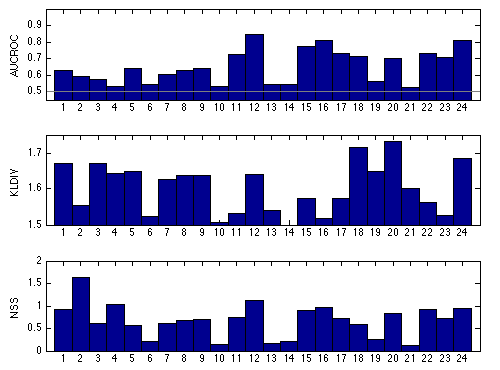
\includegraphics[width=15cm]{pics/single-accv.png}
  \caption{Vizualizácia všetkých testovaných metrík pre dataset ASCMN\cite{accv} pre jednotlivé videá}
  \label{fig:ASCMNOne}
\end{figure}

\subsubsection{ASCMN - AUCROC}
Ideálna hodnota tejto metriky je 1, čo reálne značí 100\% úspešnosť.
Náhodná mapa pozornosti má hodnotu 0.5, z toho dôvodu aby sme dokázali správnosť nového modelu potrebujeme dokázať, že model má hodnotu AUC v intervale \interval[{0.5,1}].
Z grafu \ref{fig:ASCMNOne} vyplýva, že všetky videá spĺňajú vyššie uvedenú podmienku.
Výsledná priemerná hodnota pre AUC 0.6515.
Táto hodnota už priamo dokazuje túto hypotézu, keďže ho tvorí stredná hodnota všekých testovaných videí.
Kedže je hodnota dostatočne vyššia ako 0.5. hodnota vyhodnocuje náš model ako korelujúci s reálne nameranými dátami na používateľoch zúčastnených sa na tvorbe tohoto datasetu.
\subsubsection{ASCMN - KLDIV}
Ideálna hodnota tejto metriky je 0, čo reálne značí že saliency mapa je totožná s ground truth mapou.
Výsledné hodnoty pre všetky videá sa podľa grafu \ref{fig:ASCMNOne} pohybujú v intervale \interval[{1.5,1.7}].
Hodnoty menšie ako 2 značia tiež koreláciu s reálnymi dátami.
Výsledná hodnota KLDIV je 1.6027 je nižsia ako 2, preto aj metrika KLDIV úspešne validuje náš model vrámci datasetu.
\subsubsection{ASCMN - NSS}
Výsledná hodnota NSS je 0.6809.
Hodnota NSS metriky odhaluje, že hodnoty v oblastiach fixácií minimálne s normalizovanýmy fixáciamy a model by mal zmeniť hodnoty v oblastiach fixácii.

\subsubsection{Coutrot #1}
V datasete Coutrot #1 boli z testovania vynaté videá číslo: 34, 39, 51, 5 z dôvodu chybného zdrojového videa alebo fixácií zverejnených jeho autormy, alebo nevalídnimy výsledkamy v nejakej z vypočítavaných metrík.
\begin{figure}[H]
  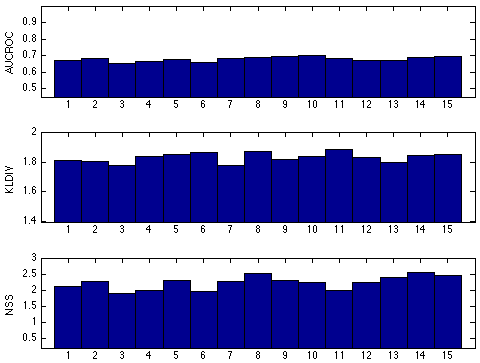
\includegraphics[width=15cm]{pics/single-coutrot1.png}
  \caption{Vizualizácia všetkých testovaných metrík pre dataset Coutrot #1\cite{coutrot-database} pre jednotlivé videá}
  \label{fig:coutrotOne}
\end{figure}
\subsubsection{Coutrot #1 - AUCROC}
Výsledná priemerná hodnota pre AUC je 0.6086.
HTakáto hodnota vyhodnocuje náš model ako korelujúci s reálne nameranými dátami na používateľoch zúčastnených sa na tvorbe tohoto datasetu.
\subsubsection{Coutrot #1 - KLDIV}
Výsledná hodnota KLDIV je 1.6280, je nižsia ako 2, preto aj metrika KLDIV úspešne validuje náš model vrámci datasetu.
\subsubsection{Coutrot #1 - NSS}
Výsledná hodnota NSS je 0.6277.
Hodnota NSS metriky odhaluje, že hodnoty v oblastiach fixácií korelujú s normalizovanýmy fixáciamy používateľov ale na tomto type videí ma model ešte rezervu.

\subsubsection{Coutrot #2}
\begin{figure}[H]
  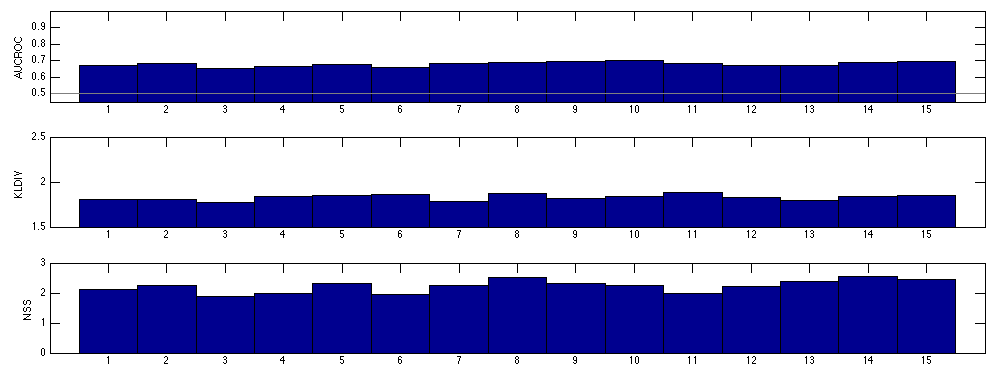
\includegraphics[width=15cm]{pics/single-coutrot2.png}
  \caption{Vizualizácia všetkých testovaných metrík pre dataset Coutrot #2\cite{coutrot-database-2} pre jednotlivé videá}
  \label{fig:coutrotTwo}
\end{figure}
\subsubsection{Coutrot #2 - AUCROC}
Výsledná priemerná hodnota pre AUC je 0.6782.
\subsubsection{Coutrot #2 - KLDIV}
Výsledná hodnota KLDIV je 1.8288 je nižsia ako 2, preto aj metrika KLDIV úspešne validuje náš model vrámci datasetu.
\subsubsection{Coutrot #2 - NSS}
Výsledná hodnota NSS je 2.2313.
Vysoká hodnota tejto metriky na tomto type videií je logickým dôvodom typu videa.
V tomto datasete bola pozornosť podla výstupných meraní užívateľov upriamená na iba málo oblastí v obraze naraz (v tomto prípade tvár alebo ruky účinkujúcich) a tímto oblastiam pridam vysokú hodnotu.
Navrhovaná métoda postupuje podobne, vyčlení pohybujúce sa oblasti (pre takýto typ videa je pohubúcich oblastí sa málo) a kedže netrovia majoritnú oblasť videa utlačí statické príznaky, čoho dôsledkom je vysoké hodnotenie týchto obastí čo odpovedá vysokej hodnote porovnávajúcej sa v metrike.

\subsubsection{Zhrnutie hodnotenia}
Pri celkovom hodnotení bude pre nás smerodajná hlavne metriky AUCROC.
Priemer pre všetky 3 testované datasety má hodnotu 0.6277 z čoho jasne výplýva úspešná validácia korelácie s nameranýmy dátamy.
Metrika KLDIV dosahuje priemernú hodnotu pre všeky datasety 1.6438. 
Metrika KLDIV poukazje na fakt ze metóda označuje viacej oblastí ako významných aj keď neboli namerané.
Metrika NSS dosahuje priemernú hodnotu pre všeky datasety 0.5487.
Táto metrika validuje, že aj hodnoty v oblastich fixácií korelujú s dátami.
V tejto metrike však záleží od typu videa viacej ako u iných metrík.

\subsection{Porovnávanie s konkurenčnými modelmi pozornosti}
Porovnanie s konkurenciou nám poskytne ďalšie relevantné poznatky.
Budeme sa konkrétne snažiť dokázať ze efektivita našeho nového modelu je vyššia ako pôvodného horn-struck algoritmu\cite{horn-schunck}, používaného na extrakciu dynamickej zložky príznakov.
Zároveň sa budem snažiť o dôkaz, že algoritmus je efektívnejší aj ako samotná statická zložka, ktorá je vypočítavaná pomocou modelu Spektralnych rezidual\cite{spectral-rezidual}.
Pre tento účel som uskutočnil benchmark obsahujúci nasledovné algoritmy:
\begin{enumerate}
  \item\textbf{AttentionSimpleGlobalRarity\cite{global-rarity}}
  \item\textbf{AttentionSimpleLocalContrast\cite{global-rarity}}
  \item\textbf{FES\cite{fes}}
  \item\textbf{RARE\cite{rare-1}}
  \item\textbf{Horn-struck\cite{horn-schunck}}
  \item\textbf{Lucas-Kanade\cite{lucas-kanade}}
  \item\textbf{Spektralne rezidua\cite{spectral-rezidual}}
\end{enumerate}
na všetkých datasetoch.
Ku každému datasetu uvedieme 2 súhrnné štatistiky.
Prvá vyjadruje porovnanie priemernej hodnoty každej z metrík pre kažkdé video samostatne, druhá obsahuje priemerné hodnoty všetkých videií, pre všetky testované medódy.

\subsubsection{ASCMN}
V ASCMN datasete bolo testovanie uskutočnené na všetkých videách a všetkých vyššie uvedených modeloch.

\begin{figure}[H]
  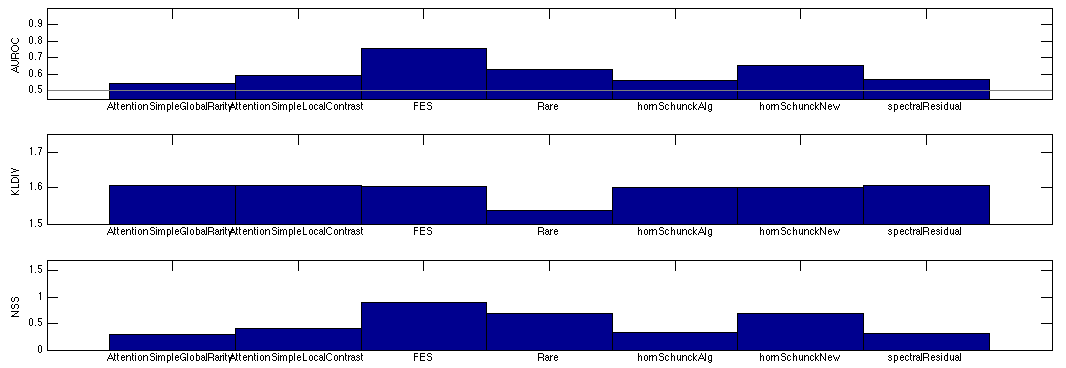
\includegraphics[width=15cm]{pics/porovnanie-accv-global-new.png}
  \caption{Vizualizácia porovnania pre dataset ASCMN\cite{accv}}
\end{figure}

\begin{figure}[H]
  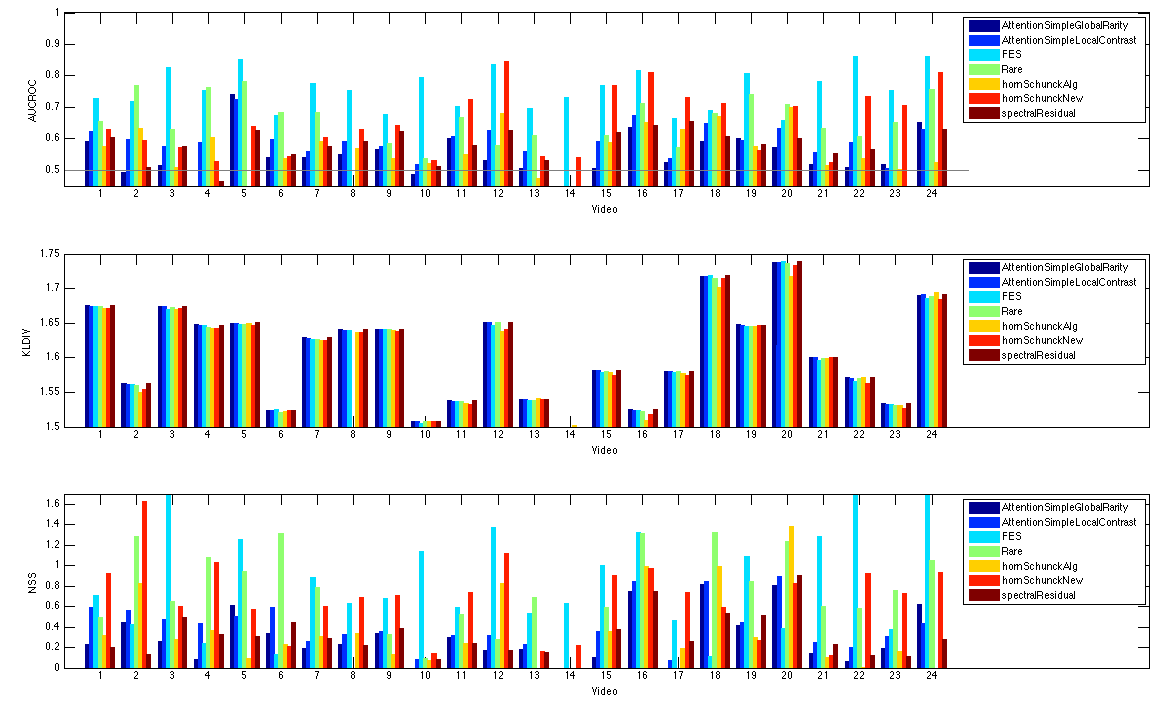
\includegraphics[angle=90, width=13cm]{pics/porovnanie-accv-new.png}
  \caption{Vizualizácia porovnania pre dataset ASCMN\cite{accv}}
\end{figure}

\subsubsection{Coutrot #1}
V datasete Coutrot #1 boli z testovania vynaté niektoré videá z dôvodu chybového spracovanie v jednom alebo viacerých testovaných modelov.
\begin{figure}[H]
  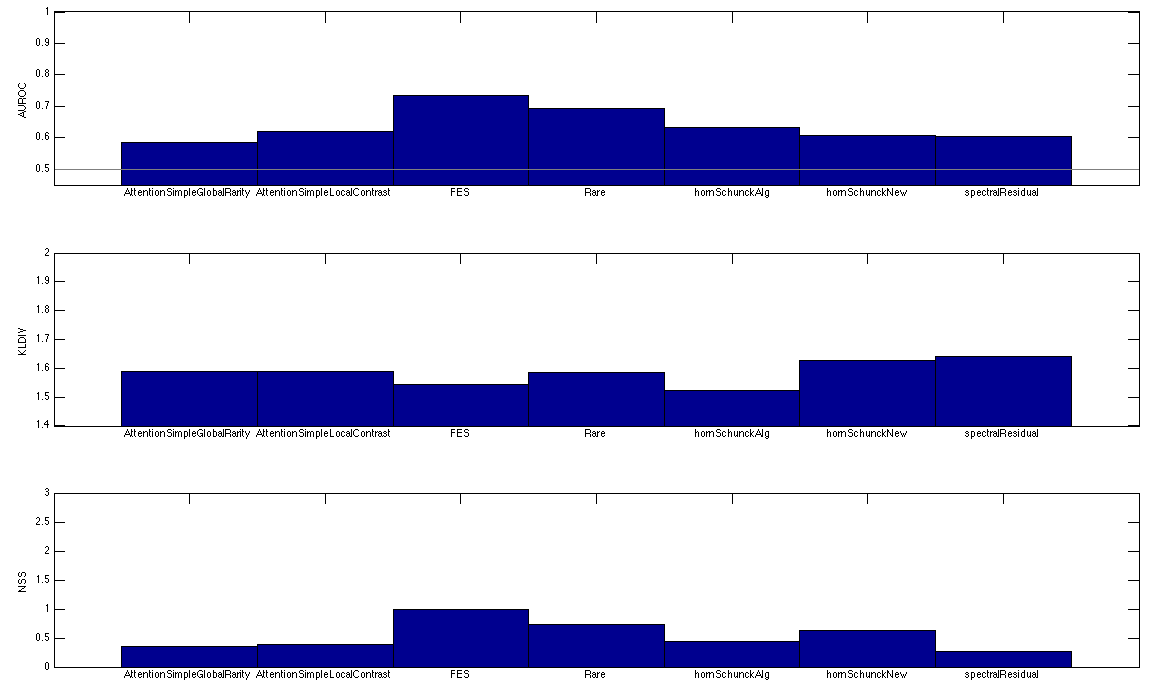
\includegraphics[width=15cm]{pics/porovnanie-coutrot1-global.png}
  \caption{Vizualizácia porovnania pre dataset Coutrot #1\cite{coutrot-database}}
\end{figure}

\begin{figure}[H]
  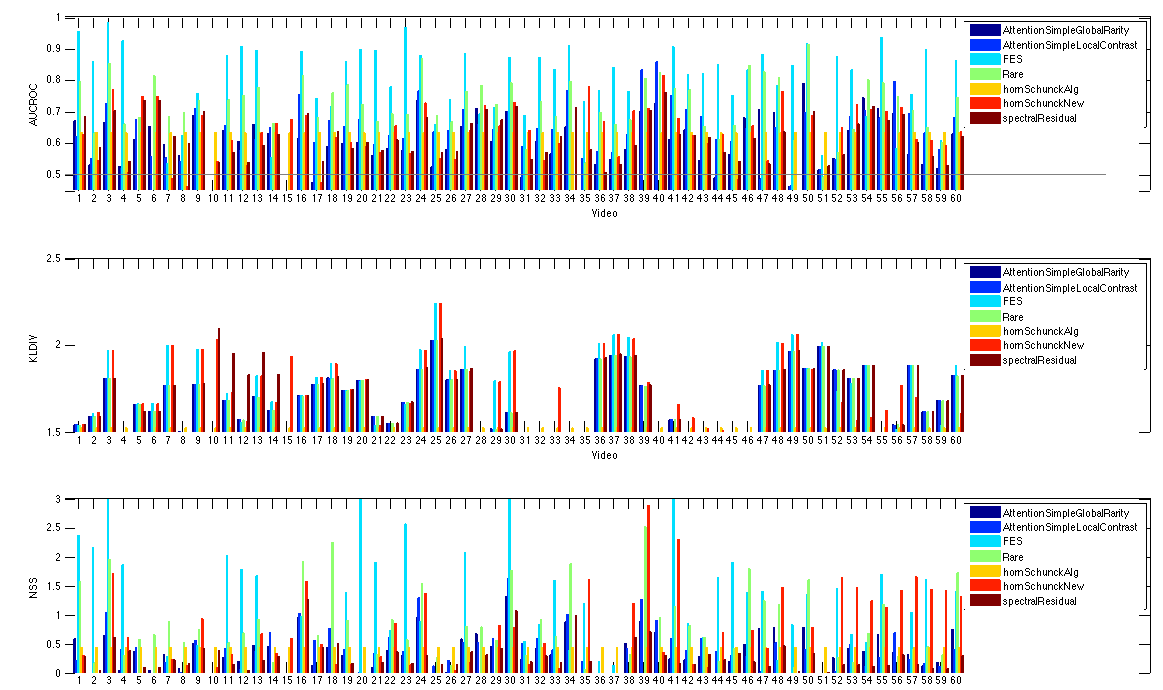
\includegraphics[angle=90, width=13cm]{pics/porovnanie-coutrot1.png}
  \caption{Vizualizácia porovnania pre dataset Coutrot #1\cite{coutrot-database}}
\end{figure}

\subsubsection{Coutrot #2}
\begin{figure}[H]
  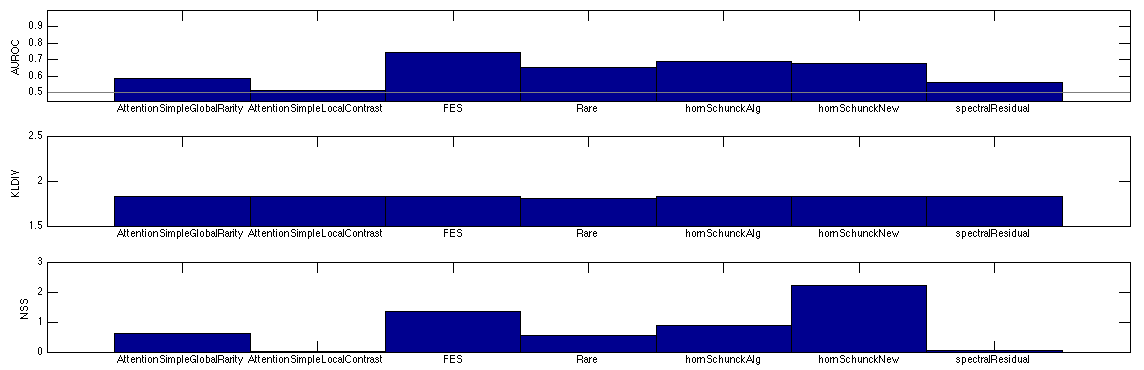
\includegraphics[width=15cm]{pics/porovnanie-coutrot2-global.png}
  \caption{Vizualizácia porovnania pre dataset Coutrot #2\cite{coutrot-database-2}}
\end{figure}

V datasete Coutrot #2 bolo testovanie uskutočnené na všetkých videách a všetkých vyššie uvedených modeloch.
\begin{figure}[H]
  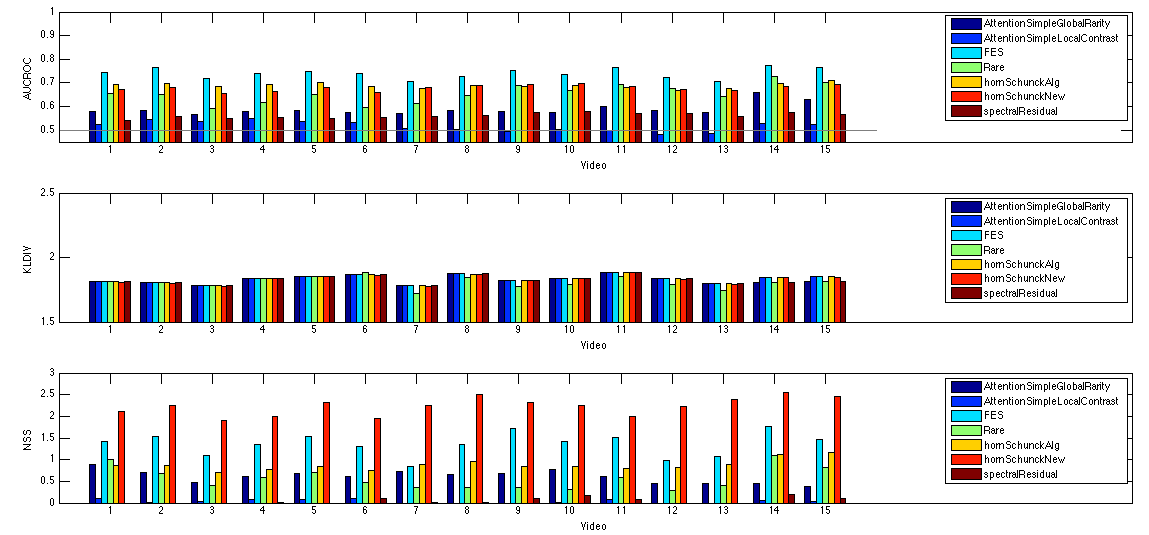
\includegraphics[angle=90, width=12cm]{pics/porovnanie-coutrot2.png}
  \caption{Vizualizácia porovnania pre dataset Coutrot #2\cite{coutrot-database-2}}
\end{figure}

\subsubsection{Zhrnutie benchmarku}
Celkové hodnotenie benchamrku znazorním porovnanním priemerov všetkých datasetov spolu.

\begin{figure}[H]
  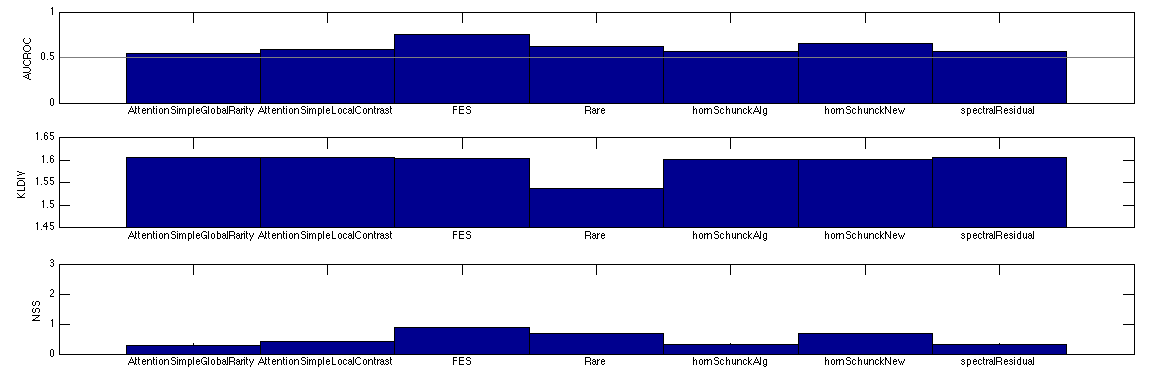
\includegraphics[width=15cm]{pics/benchmark.png}
  \caption{Vizualizácia porovnania pre všetky datasety}
\end{figure}

\subsection{Zhrnutie validacie}
Všetky metriky potvrdzujú tvrdenie, že narvhovaný model ma značnú koreláciu k skutočným dátam nameraných na reálnych užívateľoch.
Zároveň validácia bola prevedená na typovo rozdielnych videách, keďže videá obsahujú pohybujúcu sa kameru aj statickú pozíciu kamery, konverzačné scény aj scény s prírodnými motívami.
Zároveň na základe vypracovaného benchmarku možeme tvrdiť, že nová metóda je efektívnejšia vo vädšine prípadov ako obe základné metódy použité na získanie dynamických aj statických príznakov a vo všetkých videách dosahuje lepšie výsledky ako aspoň jeden zo základných algoritmov.

\section{Diskusia}
\label{ssec:diskusia}
Možnosť na zlepšenie algoritmu vidieť v celom benchmarku, kde model Rare\cite{rare-1} dosahoval výrazne lepšie výsledky aj napriek používaniu iba statických príznakov.
Preto použitie algoritmu Rare\cite{rare-1} by viedlo k zlepšeniu aktuálnych výsledkov.

\\

Ďaľšia možnosť ako vylepšiť je v rýchlosti spracovania, ktorá nie je použiteľná na realtime spracovanie videa v štandardnej kvalite videa.
Algoritmus je svojou časovou náročnosťou vhodný na spracovanie videí v nízkej obrazovej kvalite.
Avšak pri vysokej obrazovej kvalite, algoritmus nevykazoval vyššiu efektivitu (otestované na datasete savam\cite{savam} ktorý poskytuje videá vo vysokej kvalite).
Ale výpočet trval výrazne dlhšie ako v porovnaní s videom s nízkou obrazovou kvalitou.

\\

Ďaľšiu možnosť pre zlepšenie odhaľuje validácia datasetu Coutrot #2\cite{coutrot-database-2}, kde pôvodný algotritmus horn-struck dosiahol hodnotenie porovnateľné s navrhovaným modelom.
Takéto výsledky sú spôsobené výberom rozostupu frameov (podľa ktorých sa počíta dynamická zložka).
Keďže rozpätie bolo zvolené na každú dvojicu framov pri týchto videách sa často stávalo, že algoritmus detekoval iba minimálny pohyb.
Čo bolo považované za šum a z toho dôvodu bola dymamická zložka potlačená alebo úplne eliminovaná (čo bolo v tomto prípade chybné).
Riešením by bolo porovnávanie viacej framov a následná extrakcia pohybu všetkých dvojíc dokopy.
Tento postup by už nebol považovaný za šum a dynamická zložka by nebola elliminovaná.
Daľšou možnostou je použiť nejakú formu rozloženia videa na dinamicky sa meniace keyframy medzi ktorímy sa bude výpočítavať dinamická žložka mapy, zatiaľ čo statická sa bude generovať počas kažkého framu.